\section{Solving Systems}

\subsection{Composite Function Spaces}

\begin{frame}
\frametitle{Model Problem in Mixed Formulation}
Rewrite elliptic model problem as a system of first order equations:
\begin{subequations}
\label{Eq:DiffusionEquationMixedForm}
\begin{align*}
\sigma + \nabla u &= 0 & \text{in }& \Omega,\\
\nabla \cdot \sigma     &= f & \text{in }& \Omega,\\
                      u &= g& \text{on }& \Gamma_D\subseteq\partial\Omega,\\
        \sigma\cdot n  &= j& \text{on }& \Gamma_N=\partial\Omega\setminus\Gamma_D.
\end{align*}
\end{subequations}

Weak formulation. Define $H(\text{div};\Omega)$ and its subspace:
\begin{subequations}
\begin{align*}
S &= \{\sigma\in \left(L_2(\Omega)\right)^d \,|\,
\nabla\cdot \sigma \in L_2(\Omega)\}, &
\tilde{S} &= \{\sigma\in S \,|\, \text{``$\sigma\cdot n=0$'' on $\Gamma_N$} \}.
\end{align*}
\end{subequations}

Find $(\sigma,u)\in (w+\tilde{S})\times L_2(\Omega)$ ($w$ extension of $j$ !) s. t.
\begin{align*}
\int\limits_\Omega \sigma\cdot v \, dx  -\int\limits_\Omega
u \, \nabla\cdot v \, dx & =
-\int\limits_{\Gamma_D} g v\cdot n \, ds
& \forall v &\in \tilde{S}\\
- \int\limits_\Omega \nabla\cdot\sigma \, q \, dx      &=
- \int\limits_\Omega f q \, ds &
\forall q &\in L_2(\Omega)
\end{align*}
\end{frame}


\begin{frame}
\frametitle{$H(\text{div};\Omega)$ Conforming Finite Elements}
Raviart-Thomas space of lowest order on triangles is
\begin{align*}
S_h = \left\{\sigma\in\left(L_2(\Omega) \right)^2  \,\Bigl|\, \sigma|_{\Omega_e} =
\left(\begin{array}{l} a_e\\ b_e \end{array}\right) +
c_e \left(\begin{array}{l} x\\ y \end{array}\right) \quad\forall e\in E^0_h
\right\}
\end{align*}
with subspace $\tilde{S}_h = \{\sigma_h\in S_h \,|\, \text{``$\sigma_h\cdot n=0$'' on $\Gamma_N$} \}$.

Define the residual form
\begin{equation*}
\begin{split}
r^\text{mixed}((\sigma,u)&,(v,q)) =
\int\limits_\Omega \sigma\cdot v \, dx  -\int\limits_\Omega
u \, \nabla\cdot v \, dx
 - \int\limits_\Omega \nabla\cdot\sigma \, q \, dx\\
&\quad + \int\limits_{\Gamma_D} g v\cdot n \, ds + \int\limits_\Omega f q \,
ds .
\end{split}
\end{equation*}
Discrete problem in residual form reads
\begin{equation*}
(\sigma_h, u_h) \in (w_h+\tilde{S}_h)\times W_h : \quad
r_h^\text{mixed}\left((\sigma_h,u_h),(v,q)\right) = 0 \quad \forall
(v,q) \in \tilde{S}_h\times W_h .
\end{equation*}
\textbf{Systems of PDEs lead to cartesian products of function spaces !}
\end{frame}

\begin{frame}
\frametitle{Function Space Composition}
Given $k>1$ function spaces $U_0, \ldots, U_{k-1}$ we define the
composite function space
\begin{equation*}
U = U_0 \times U_1 \times \ldots \times U_{k-1} .
\end{equation*}

If all component spaces are the same we can also write
\begin{equation*}
U = V^k
\end{equation*}

This can be done \textit{recursively}. E.g. for solving the Stokes equation
in dimension $d$ using Taylor-Hood elements we would require
\begin{equation*}
U_h^\text{TH} = \left( U_h^2\right)^d \times U_h^1
\end{equation*}

Composite function spaces have tree structure:
\begin{minipage}[c]{0.2\textwidth}
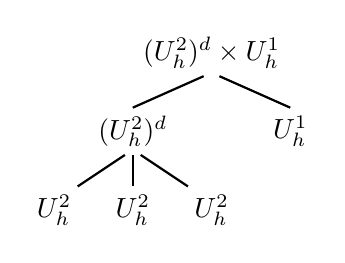
\begin{tikzpicture}[scale=1.0]
\draw (0,0) node {$U_h^2$};
\draw (1,0) node {$U_h^2$};
\draw (2,0) node {$U_h^2$};
\draw (1,1) node {$(U_h^2)^d$};
\draw (2,2) node {$(U_h^2)^d\times U_h^1$};
\draw (3,1) node {$U_h^1$};
\draw[thick] (0.3,0.3) -- (0.9,0.7);
\draw[thick] (1,0.3) -- (1,0.7);
\draw[thick] (1.7,0.3) -- (1.1,0.7);
\draw[thick] (1,1.3) -- (1.9,1.7);
\draw[thick] (3,1.3) -- (2.1,1.7);
\end{tikzpicture}
\end{minipage}
\end{frame}

\begin{frame}
\frametitle{Implementation of Function Space Composition}
\begin{itemize}
\item \lstinline{Dune::PDELab::PowerGridFunctionSpace<GFS,k,VBE,OT>} builds a
new grid function space that is \lstinline{k}-times the product of \lstinline{GFS}.\\
\lstinline{VBE} is a vector backend, \lstinline{OT} is an ordering tag.
\item \lstinline{D...::CompositeGridFunctionSpace<VBE,OT,GFS0,...,GFSk>}
builds a new grid function space out of the given grid function
spaces.
\item \lstinline{OT} controls construction of local to global map, allowing e.g. block-wise or component-wise ordering.
\item This can be applied recursively leading to a type tree.
\item Leaves of the tree are scalar or vector-valued finite element spaces.
\item The local function spaces given to local operators reflects this tree structure.
\item \lstinline{Dune::PDELab::GridFunctionSubSpace} allows the selection of subspaces.
\item User functions (e.g. for initial conditions) can be composed in a similar way.
\end{itemize}
\end{frame}

Now the Taylor-Hood interpolation example.

\begin{frame}<presentation>[fragile,allowframebreaks,allowdisplaybreaks]
\frametitle<presentation>{Taylor Hood Example Listing}
\framesubtitle<presentation>{File \texttt{src/course-gridfunctionspace/thinterpolate.hh}}
\lstinputlisting[basicstyle=\tiny,numbers=left,
numberstyle=\tiny, numbersep=2pt]{../../src/course-gridfunctionspace/thinterpolate.hh}
\end{frame}
\mode<article>{
\begin{Lst}[File src/course-gridfunctionspace/thinterpolate.hh] \mbox
\nopagebreak
\lstinputlisting[basicstyle=\scriptsize,numbers=left,
numberstyle=\tiny, numbersep=2pt]{../../src/course-gridfunctionspace/thinterpolate.hh}
\end{Lst}}

\begin{frame}<presentation>
\frametitle<presentation>{Visualization of Taylor-Hood Function}
\begin{center}
\includegraphics[width=0.5\textwidth]{./EPS/thinterpolate}
\end{center}
\end{frame}

\mode<article>{
\begin{figure}
\begin{center}
\includegraphics[width=0.5\textwidth]{./EPS/thinterpolate}
\end{center}
\caption{Visualization of velocity field and pressure in the
Taylor-Hood example.}
\label{fig:THInterpolation}
\end{figure}
Figure \ref{fig:THInterpolation} visualizes the result of this
example.
}

\begin{frame}<presentation>[fragile,allowframebreaks,allowdisplaybreaks]
\frametitle<presentation>{Analytic Velocity Field Listing}
\framesubtitle<presentation>{File \texttt{src/course-gridfunctionspace/thvelocity.hh}}
For completeness here is the definition of the analytic velocity field.
\lstinputlisting[basicstyle=\tiny,numbers=left,
numberstyle=\tiny, numbersep=2pt]{../../src/course-gridfunctionspace/thvelocity.hh}
\end{frame}
\mode<article>{
For completeness here is the definition of the analytic velocity field for interpolation.
\begin{Lst}[File src/course-gridfunctionspace/thvelocity.hh] \mbox
\nopagebreak
\lstinputlisting[basicstyle=\scriptsize,numbers=left,
numberstyle=\tiny, numbersep=2pt]{../../src/course-gridfunctionspace/thvelocity.hh}
\end{Lst}}

\subsection{Example 5}

\begin{frame}
\frametitle{Problem Definition}
We solve a two-component diffusion-reaction problem with FitzHugh-Nagumo
reaction\footnote{\url{http://en.wikipedia.org/wiki/Reaction-diffusion_system}}:
\begin{subequations}
\begin{align*}
\partial_t u_0 - d_0 \Delta u_0 - f(u_0) + \sigma u_1 &= 0 &&\text{in $\Omega=(0,2)^2$},\\
\tau\partial_t u_1 - d_1 \Delta u_1 - u_0 + u_1 &= 0 &&\text{in $\Omega$},\\
\nabla u_0 \cdot n = \nabla u_1 \cdot n &= 0 &&\text{on $\partial\Omega$},\\
u_0(\cdot,t_0) &= U_0(\cdot), \\
u_1(\cdot,t_0) &= U_1(\cdot),
\end{align*}
\end{subequations}
with $f(u) = \lambda u - u^3 - \kappa$.
We will combine
\begin{itemize}
\item Conforming finite elements: $Q_1$, $Q_2$.
\item Various implicit time discretizations.
\item Newton's method.
\end{itemize}
\end{frame}

\begin{frame}
\frametitle{Example 5 Overview}
Example 5 solves the diffusion reaction problem with conforming finite elements.

It consists of the following files:
\begin{itemize}
\item \lstinline{example05.cc} -- the file to be compiled, main function.
\item \lstinline{example05_QkQk.hh} -- driver using $Q_1$ or $Q_2$ elements.
\item \lstinline{example05_operator.hh} -- local operator for spatial part.
\item \lstinline{example05_toperator.hh} -- local operator for temporal part.
\item \lstinline{example05_initial.hh} -- set up initial conditions.
\end{itemize}
\end{frame}

\begin{frame}
\frametitle{Main Features of the Driver}
\framesubtitle{About \lstinline{example05_QkQk.hh}}
\begin{itemize}
\item Make a product grid function space with two components.
\item Use \lstinline{EntityBlockedOrderingTag} to order
both degrees of freedom of the system consecutively.
\item Local operator of the system takes a number of parameters.
\item Graphical output requires subspaces to extract the components (well, if
you do not use \lstinline{addSolutionToVTKWriter}).
\item Start with small time steps that are increased progressively.
\end{itemize}
\end{frame}

\begin{frame}<presentation>[fragile,allowframebreaks,allowdisplaybreaks]
\frametitle<presentation>{Driver Using $Q_1$ Elements}
\framesubtitle<presentation>{File \texttt{src/course-examples/example05\_QkQk.hh}}
\lstinputlisting[basicstyle=\tiny,numbers=left,
numberstyle=\tiny, numbersep=2pt]{../../src/course-examples/example05_QkQk.hh}
\end{frame}
\mode<article>{
\begin{Lst}[File src/course-examples/example05\_QkQk.hh] \mbox
\nopagebreak
\lstinputlisting[basicstyle=\scriptsize,numbers=left,
numberstyle=\tiny, numbersep=2pt]{../../src/course-examples/example05_QkQk.hh}
\end{Lst}}

\begin{frame}
\frametitle{New Features of the Local Operators}
\framesubtitle{About \lstinline{example05_operator.hh}, \lstinline{example05_toperator.hh}}
\begin{itemize}
\item Local function spaces (trial and test) are now composite as well.
\item They have the same structure as the global function spaces.
\item Components are extracted with template magic according to the tree structure.
%\item \lstinline{localIndex()} method on local function space maps
%a degree of freedom from this space to all degrees of freedom of the element.
\item The \lstinline{x} and \lstinline{r} arguments allow access to the individual components.
\item This local operator would work also when $u_0$ and $u_1$ are discretized
with different finite element spaces.
\item Same features are used in the temporal part.
\end{itemize}
\end{frame}

\begin{frame}<presentation>[fragile,allowframebreaks,allowdisplaybreaks]
\frametitle<presentation>{Local Operator Spatial Part}
\framesubtitle<presentation>{File \texttt{src/course-examples/example05\_operator.hh}}
\lstinputlisting[basicstyle=\tiny,numbers=left,
numberstyle=\tiny, numbersep=2pt]{../../src/course-examples/example05_operator.hh}
\end{frame}
\mode<article>{
\begin{Lst}[File src/course-examples/example05\_operator.hh] \mbox
\nopagebreak
\lstinputlisting[basicstyle=\scriptsize,numbers=left,
numberstyle=\tiny, numbersep=2pt]{../../src/course-examples/example05_operator.hh}
\end{Lst}}

\begin{frame}<presentation>[fragile,allowframebreaks,allowdisplaybreaks]
\frametitle<presentation>{Local Operator Temporal Part}
\framesubtitle<presentation>{File \texttt{src/course-examples/example05\_toperator.hh}}
\lstinputlisting[basicstyle=\tiny,numbers=left,
numberstyle=\tiny, numbersep=2pt]{../../src/course-examples/example05_toperator.hh}
\end{frame}
\mode<article>{
\begin{Lst}[File src/course-examples/example05\_toperator.hh] \mbox
\nopagebreak
\lstinputlisting[basicstyle=\scriptsize,numbers=left,
numberstyle=\tiny, numbersep=2pt]{../../src/course-examples/example05_toperator.hh}
\end{Lst}}

\begin{frame}<presentation>
\frametitle{Visualization of Example 5 Results}
\begin{center}
\includegraphics[width=0.3\textwidth]{./EPS/example05_0_05} $\hspace{1mm}$
\includegraphics[width=0.3\textwidth]{./EPS/example05_0_5} $\hspace{1mm}$
\includegraphics[width=0.3\textwidth]{./EPS/example05_0_50}\\
\includegraphics[width=0.3\textwidth]{./EPS/example05_1_05} $\hspace{1mm}$
\includegraphics[width=0.3\textwidth]{./EPS/example05_1_5} $\hspace{1mm}$
\includegraphics[width=0.3\textwidth]{./EPS/example05_1_50}\\
{\tiny $t=0.5$ \hspace{30mm} $t=5.0$ \hspace{30mm} $t=50.0$}
\end{center}
\end{frame}

\mode<article>{
Figure \ref{fig:Example05Results} shows visualizations of the results computed
with \lstinline{example05}.
\begin{figure}
\begin{center}
\includegraphics[width=0.3\textwidth]{./EPS/example05_0_05} $\hspace{1mm}$
\includegraphics[width=0.3\textwidth]{./EPS/example05_0_5} $\hspace{1mm}$
\includegraphics[width=0.3\textwidth]{./EPS/example05_0_50}

\medskip

\includegraphics[width=0.3\textwidth]{./EPS/example05_1_05} $\hspace{1mm}$
\includegraphics[width=0.3\textwidth]{./EPS/example05_1_5} $\hspace{1mm}$
\includegraphics[width=0.3\textwidth]{./EPS/example05_1_50}
\end{center}
\caption{Results for example 5 computed with $Q_1$ elements on a $128\times 128$ grid
at times $0.5, 5$ and $50$ (left to right) and components 0 and 1 (top to bottom).
Parameters of the FitzHugh-Nagumo model were $d_0=0.00028$, $d_1=0.005$,
$\lambda=1$, $\sigma=1$, $\kappa=-0.05$ and $\tau=0.1$.}
\label{fig:Example05Results}
\end{figure}
}

\begin{frame}<presentation>
\frametitle{Example 5 Animations}
\begin{center}
\movie{\includegraphics[width=0.48\textwidth]{./EPS/turing}}{turing.avi}$\hspace{1mm}$
\movie{\includegraphics[width=0.48\textwidth]{./EPS/turing_3D}}{turing_3D.avi}
\end{center}
\end{frame}


\subsection{Example 6}

\begin{frame}
\frametitle{Example 6 Overview}
We demonstrate orthogonality of concepts by parallelizing example 5.

Example 6 consist of the following files
\begin{itemize}
\item \lstinline{example06.cc} -- the file to be compiled, main function.
\item \lstinline{example06_Q1Q1.hh} -- parallel driver for \textit{overlapping} grids.
\item \lstinline{example06_bctype.hh} -- dummy boundary condition type for overlapping constraints class.
\end{itemize}
\end{frame}

\begin{frame}
\frametitle{Main Features of the Parallel Driver}
\framesubtitle{About \lstinline{example06_Q1Q1.hh}}
\begin{itemize}
\item Needs \lstinline{OverlappingConformingDirichletConstraints}
to assemble Dirichlet constraints at artificial processor boundaries.
\item Needs boundary condition type function to call \lstinline{constraints()} function.
\item Operators and initial conditions are taken from example 5.
\item Select a parallel solver backend for overlapping grids.
\item Invoke driver with a parallel overlapping grid (see \lstinline{example06.cc}).
\item Thats it.
\end{itemize}
\end{frame}

\begin{frame}<presentation>[fragile,allowframebreaks,allowdisplaybreaks]
\frametitle<presentation>{Parallel Instationary Nonlinear Driver}
\framesubtitle<presentation>{File \texttt{src/course-examples/example06\_Q1Q1.hh}}
\lstinputlisting[basicstyle=\tiny,numbers=left,
numberstyle=\tiny, numbersep=2pt]{../../src/course-examples/example06_Q1Q1.hh}
\end{frame}
\mode<article>{
\begin{Lst}[File src/course-examples/example06\_Q1Q1.hh] \mbox
\nopagebreak
\lstinputlisting[basicstyle=\scriptsize,numbers=left,
numberstyle=\tiny, numbersep=2pt]{../../src/course-examples/example06_Q1Q1.hh}
\end{Lst}}

\begin{frame}
\frametitle{Further Examples for Local Operators}
in \lstinline{dune/pdelab/localoperator} you find
\begin{itemize}
\item \lstinline{convectiondiffusionfem.hh} -- stationary convection-diffusion equation with variable full tensor using
continuous Galerkin method.
\item \lstinline{convectiondiffusiondg.hh} -- stationary convection-diffusion equation with variable full tensor using discontinuous
Galerkin method.
\item \lstinline{diffusionmixed.hh} -- variable coefficient diffusion problem using $RT0$ mixed method.
\item \lstinline{linearacousticsdg.hh} -- equations of linear acoustics using discontinuous Galerkin.
\item \lstinline{maxwelldg.hh} -- Maxwell's equations using discontinuous Galerkin.
\item \lstinline{twophaseccfv.hh} -- water-gas flow in porous media using pressure-pressure formulation,
cell-centered finite volumes.
\end{itemize}
\ldots and more.
\end{frame}


\cleardoublepage
